%\documentclass[12pt,a4]{revtex4}
%\documentclass[12pt]{article}
%\documentclass[11pt, twocolumn]{article}
\documentclass[12pt,notitlepage,aps,pra,longbibliography,nofootinbib,tightenlines,superscriptaddress]{revtex4}

%\usepackage{epsf}
\usepackage{amsmath}
\usepackage{color}

%\documentclass[12pt,a4]{revtex4}
%\documentclass[12pt]{article}
%\documentclass[11pt, twocolumn]{article}

%\usepackage{epsf}
\usepackage{amsmath}
\usepackage{color}
\usepackage{natbib}
\usepackage{wrapfig}
%\usepackage{cite}



\RequirePackage{amsmath}
\RequirePackage{amssymb}
\RequirePackage{amsthm}
%\RequirePackage{algorithmic}
%\RequirePackage{algorithm}
%\RequirePackage{theorem}
%\RequirePackage{eucal}
\RequirePackage{color}
\RequirePackage{url}
\RequirePackage{mdwlist}

\RequirePackage[all]{xy}
\CompileMatrices
\RequirePackage{hyperref}
\RequirePackage{graphicx}
%\RequirePackage[dvips]{geometry}

\def\Xcite#1{}

\def\heading #1{\vskip 20pt \noindent\underline{\large \bf #1}\vskip 5pt}

\def\important #1{\underline{\bf #1}}



\begin{document}

\title{Error Correction in a Fibonacci Anyon Code}

%\author{Simon Burton, Courtney G. Brell, Steven T. Flammia}
%\affiliation{Centre for Engineered Quantum Systems, School of Physics, The University of Sydney, Sydney, Australia}


\author{Simon Burton}
\affiliation{Centre for Engineered Quantum Systems, School of Physics, The University of Sydney, Sydney, Australia}
\author{Courtney G.\ Brell}
\affiliation{Centre for Engineered Quantum Systems, School of Physics, The University of Sydney, Sydney, Australia}
\affiliation{Institut f\"ur Theoretische Physik, Leibniz Universit\"at Hannover, Appelstra\ss e 2, 30167 Hannover, Germany}
\author{Steven T.\ Flammia}
\affiliation{Centre for Engineered Quantum Systems, School of Physics, The University of Sydney, Sydney, Australia}


%\begin{abstract}
%We consider two dimensional
%systems that support Fibonacci
%anyon excitations.
%These are phenomenological models in that
%we ignore microscopic structure such as
%any underlying spin model.
%In our system the vacuum state of a torus
%is two-fold degenerate and we use this as a
%one qubit code.
%The error model consists of iid pair-creation
%processes for some varying amount of time.
%Error correction proceeds by first measuring
%a syndrome: this is the total charge in each
%tile of some tiling of the surface.
%The (classical) error correction algorithm
%performs repeated hierarchical clustering (fusing) of anyons,
%until there are no more charges remaining.
%This fails (destroys the encoded state)
%exactly when a topologically non-trivial operation occurs.
%Note that the error correction algorithm runs in polynomial time,
%but the simulation of the anyon system naively takes exponential
%time (and memory.) Here we find that a divide and conquer approach,
%as well as heuristics to minimise braid operations, allow
%simulation of systems to a reasonably large size (128x128 tiles),
%and we observe an error correction threshold of around $12.5\%$.
%\end{abstract}


\maketitle

%\heading{Introduction}


\important{Introduction.}
Topologically ordered systems in two dimensions are of great interest  
for quantum information processing and storage. These systems can be  
realized as ground states of local Hamiltonians and have natural  
robustness to local Hamiltonian perturbations~\cite{Bravyi2010,  
Bravyi2011a, Michalakis2013}. Furthermore, these systems typically  
have anyonic excitations~\cite{Wilczek1990, Kitaev2006} that may be  
used to realize fault-tolerant quantum computation by braiding of  
these particles~\cite{Kitaev2003, Nayak2008}. Different topologically  
ordered systems have different anyonic excitations, but only anyon  
models with sufficient complexity can be used to perform universal  
quantum computation in this way.

The Fibonacci anyon model is one of the simplest abstract anyon models  
to describe, having only one non-trivial particle type. Nonetheless,  
it allows for universal quantum computation by braiding~\cite{Freedman2002} and so  
is of great theoretical interest. Furthermore, the Fibonacci anyons  
are experimentally motivated as the expected excitations of the  
$\nu=\frac{12}{5}$ fractional quantum Hall states~\cite{Slingerland2001}, and can  
also be realized in several spin models~\cite{Levin2005, Palumbo2013, Kapit2013}.


Any scheme using anyon braiding to perform quantum computation will  
periodically require some form of active error correction to remove  
spurious thermal excitations. Left unchecked, the computation will  
quickly be spoiled at finite temperature. Such error-correction  
schemes have been well-developed for the simple class of abelian anyon  
models~\cite{Dennis2002,Duclos-Cianci2010a,Bravyi2011}, where only trivial computation can be performed by  
braiding.
Recently, the first error-correction schemes for non-abelian  
anyon models were proposed and demonstrated~\cite{Wootton2013, Brell2013}.
These schemes  
were developed for particular anyon models that cannot be used for  
universal quantum computation by braiding of anyons alone. This lack  
of computational power was in fact a motivating feature of the study  
of these models, as the anyon dynamics can be efficiently simulated on  
a classical computer.
By contrast, the fact that the Fibonacci anyons  
can realize universal quantum computation makes the direct  
simulation of these anyons on a classical computer decidedly  
inefficient.

%In this work we focus on demonstrating one of the main claims
%of topological quantum computing:
%that the effects of local noise
%can be overcome using error correction techniques.
In this work we use monte-carlo simulations of a 
phenomenological model.
This ignores any microscopic structure such as
an underlying lattice of spins.
The two dimensional manifold of our model has the global 
geometry of a torus which supports a two-fold degenerate
vacuum state.
This space is the codespace.
The noise model consists of iid pair-creation
events for some varying amount of time.
Error correction proceeds by first measuring
a syndrome: this is the total charge in each
tile of some tiling of the surface.
The (classical) error correction algorithm
performs repeated hierarchical clustering (fusing) of anyons,
until there are no more charges remaining.
This fails, destroying the encoded state,
exactly when a topologically non-trivial operation occurs.
Note that the error correction algorithm runs in polynomial time,
but the simulation of the anyon system naively takes exponential
time and memory.
Here we find that a divide and conquer approach,
as well as heuristics to minimise braid operations, allow
simulation of systems to a reasonably large size (128x128 tiles),
and we observe an error correction threshold of around $12.5\%$.


\important{Simulation.}
Unlike Ising anyon systems \cite{Brell2013},
Fibonacci anyon dynamics are known to be sufficient
for quantum computing \cite{Freedman2002}.
In particular, the dimension of the Hilbert
space associated with $n$ anyons
grows like $d^n$ where $d$ is the quantum
dimension of the anyons, in this case $d\simeq 1.6.$
Furthermore, the action of braiding Fibonacci 
anyons generates a dense
set of unitaries on this space (for $n>2$).
Therefore, at first sight it would appear that
we should not expect to be able to simulate
something as complicated as a decoding threshold.
However, we benefit from the following 
good fortune:

{\it (1)} below (bond) percolation threshold, we
expect the system to decompose into 
separate clusters of average size
$O(log(n))$ and variance $O(1)$, \cite{Bazant2000}.
Taking advantage of this, the simulation
proceeds by maintaining a set of disjoint
sub-systems. In other words: it is a (tensor) product
state, so we compute with each factor
separately.

{\it (2)} 
even though the act of error correction ({\it decoding})
joins these clusters together, every fusion also
decreases the number of anyons present. Moreover,
the goal of the error correction algorithm is to do this as
much as possible.

%\heading{Simulation}

We cover the surface of the torus with LxL disjoint squares.
These {\it tiles} are the regions over which
charge measurements occur, in order to
produce a syndrome for the decoder.

In order to keep track of the observables of the
system we maintain a set of disjoint {\it curves}.
These curves can also be thought of as a top-down
view of the fusion tree. In general, this winds around
the two dimensional tiles in a haphazard way determined by the
progress of the simulation.
For comparison,
previous work used a single fixed Z-shaped curve (row-major ordering)
\cite{Brell2013}.


%\begin{wrapfigure}{l}{0.26\textwidth}
%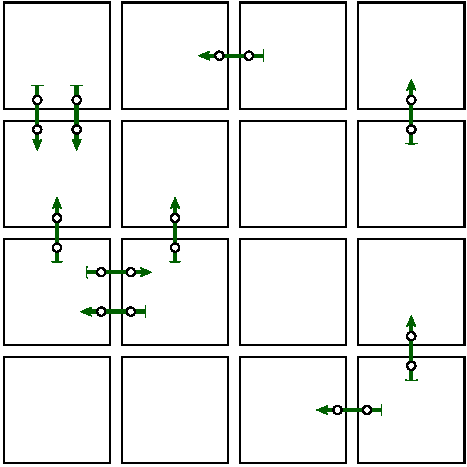
\includegraphics[width=0.26\textwidth]{pair-create.pdf}
%\end{wrapfigure}

\begin{center}
(i)
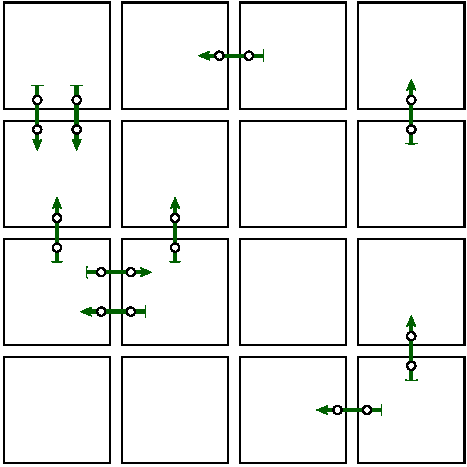
\includegraphics[width=0.26\textwidth]{pair-create.pdf}
\hskip 10pt
(ii)
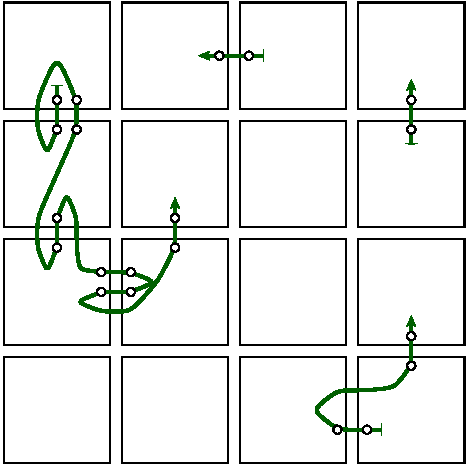
\includegraphics[width=0.26\textwidth]{syndrome-1.pdf}
\hskip 10pt
(iii)
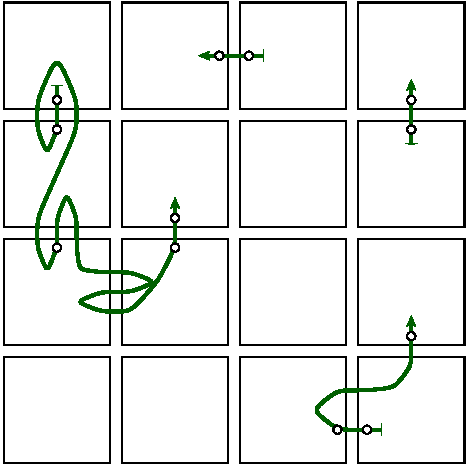
\includegraphics[width=0.26\textwidth]{syndrome-2.pdf}
\end{center}

Each round of simulation proceeds in four steps as follows:

(i) The noise process is modeled by
a sequence of pair-creation events distributed as
a Poisson process across each edge.

(ii) We first
join curves that participate in the same tile
in order to,

(iii) measure the charge on each tile.
Any resulting anyon is left somewhere in the tile.

(iv) The decoder examines this syndrome and clusters
nearby anyons. Each cluster is then measured (fused),
%and then we repeat this step clustering on a larger length
%scale.
and the decoder continues to cluster and fuse on larger scales until
there are no more anyons, or a non-trivial operation has occurred.
The non-trivial operations are those that involve a path that wraps
around the torus. All of these alter the encoded
state, and so in this case we abandon the
simulation round and declare failure to error correct.
This decoding algorithm is based on the clustering ``RG''
algorithm~\cite{Bravyi2011}.

\newpage

\important{Numerical Results}
We plot the performance of the decoder as a function
of error rate for varying lattice sizes.
The error rate is parameterized by the Poisson process duration $t_{\mathrm{sim}}$.
There is clear evidence of a decoding threshold below
which decoding succeeds with asymptotic certainty as the
system size increases.
This threshold is at $t_{\mathrm{sim}}\simeq 0.125 \pm 0.003.$

\begin{center}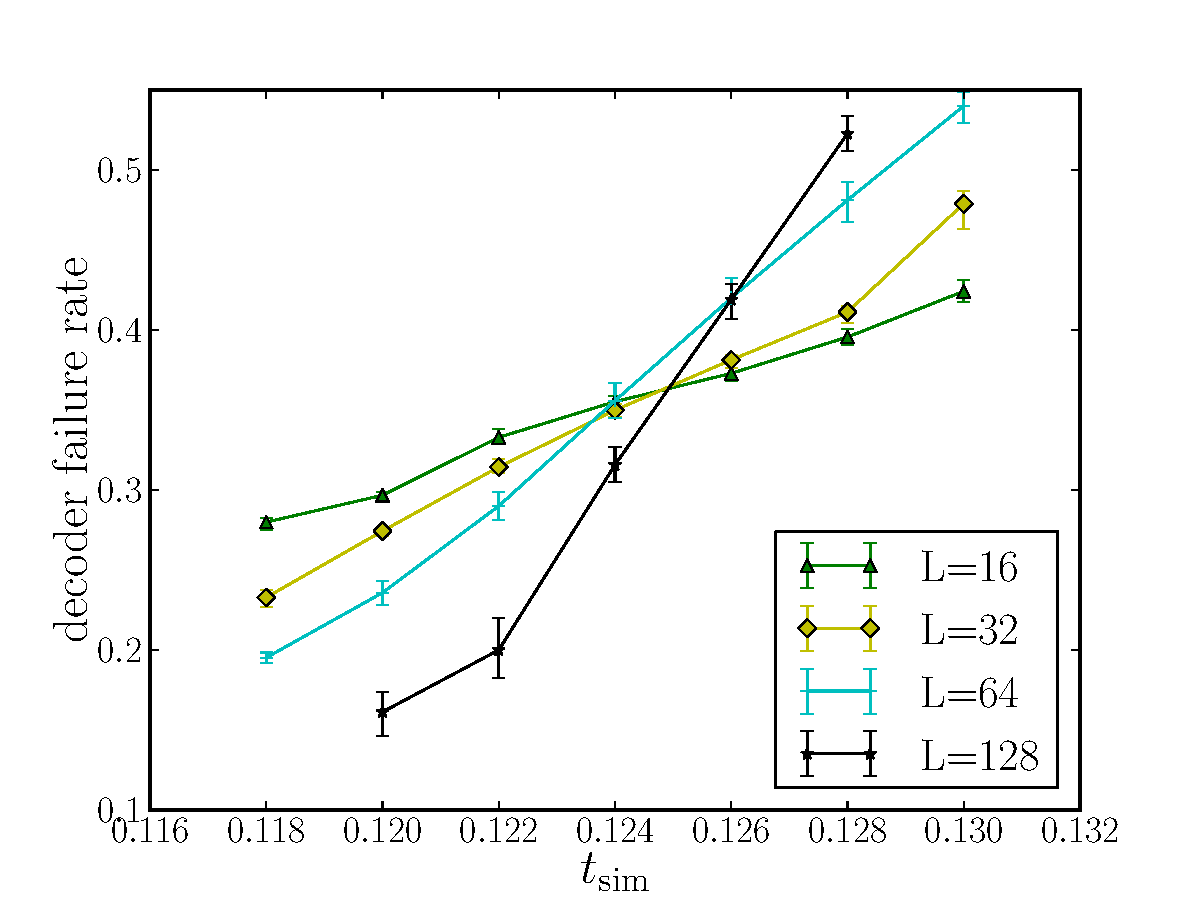
\includegraphics[width=0.6\textwidth]{anyons-kyle.pdf}\end{center}


\bibliography{refs2}{}
\bibliographystyle{abbrv}

\end{document}




